\begin{figure}[htpb]
        \centering
    \begin{subfigure}{\textwidth}
        \centering
        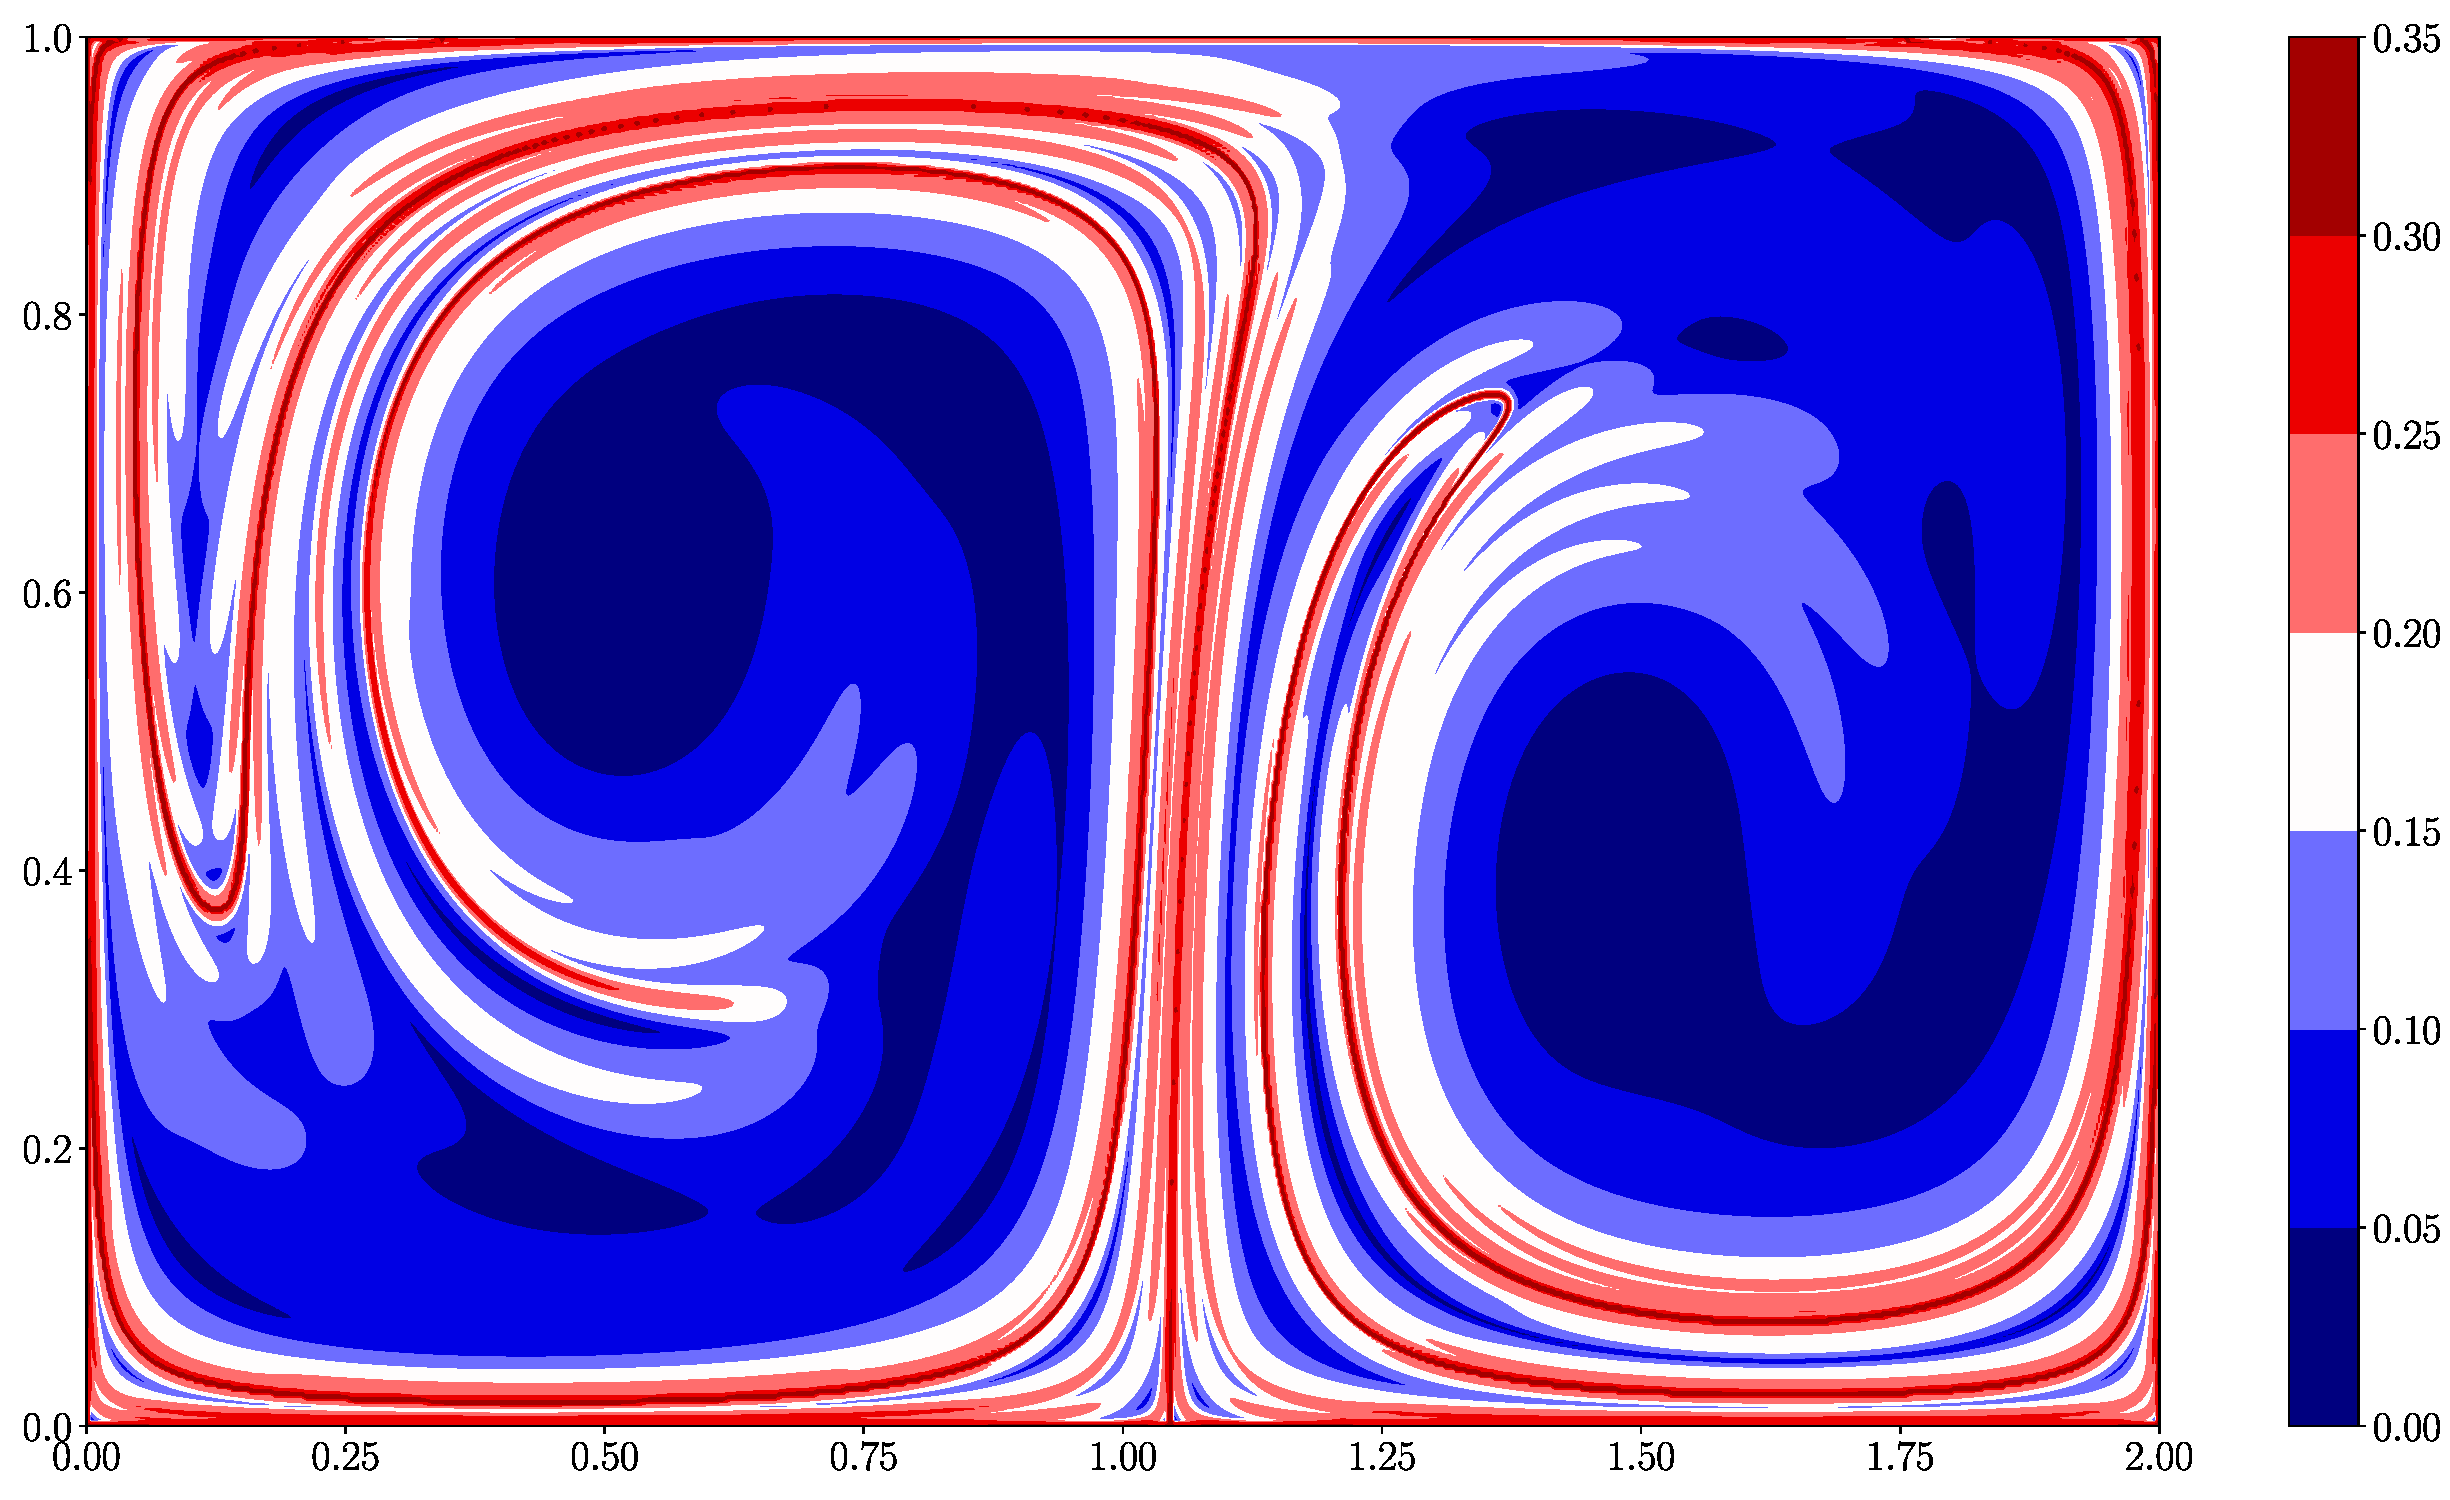
\includegraphics[width=0.75\linewidth,keepaspectratio]{figures/ftle.pdf}
    \end{subfigure}

    \begin{subfigure}{\textwidth}
        \centering
        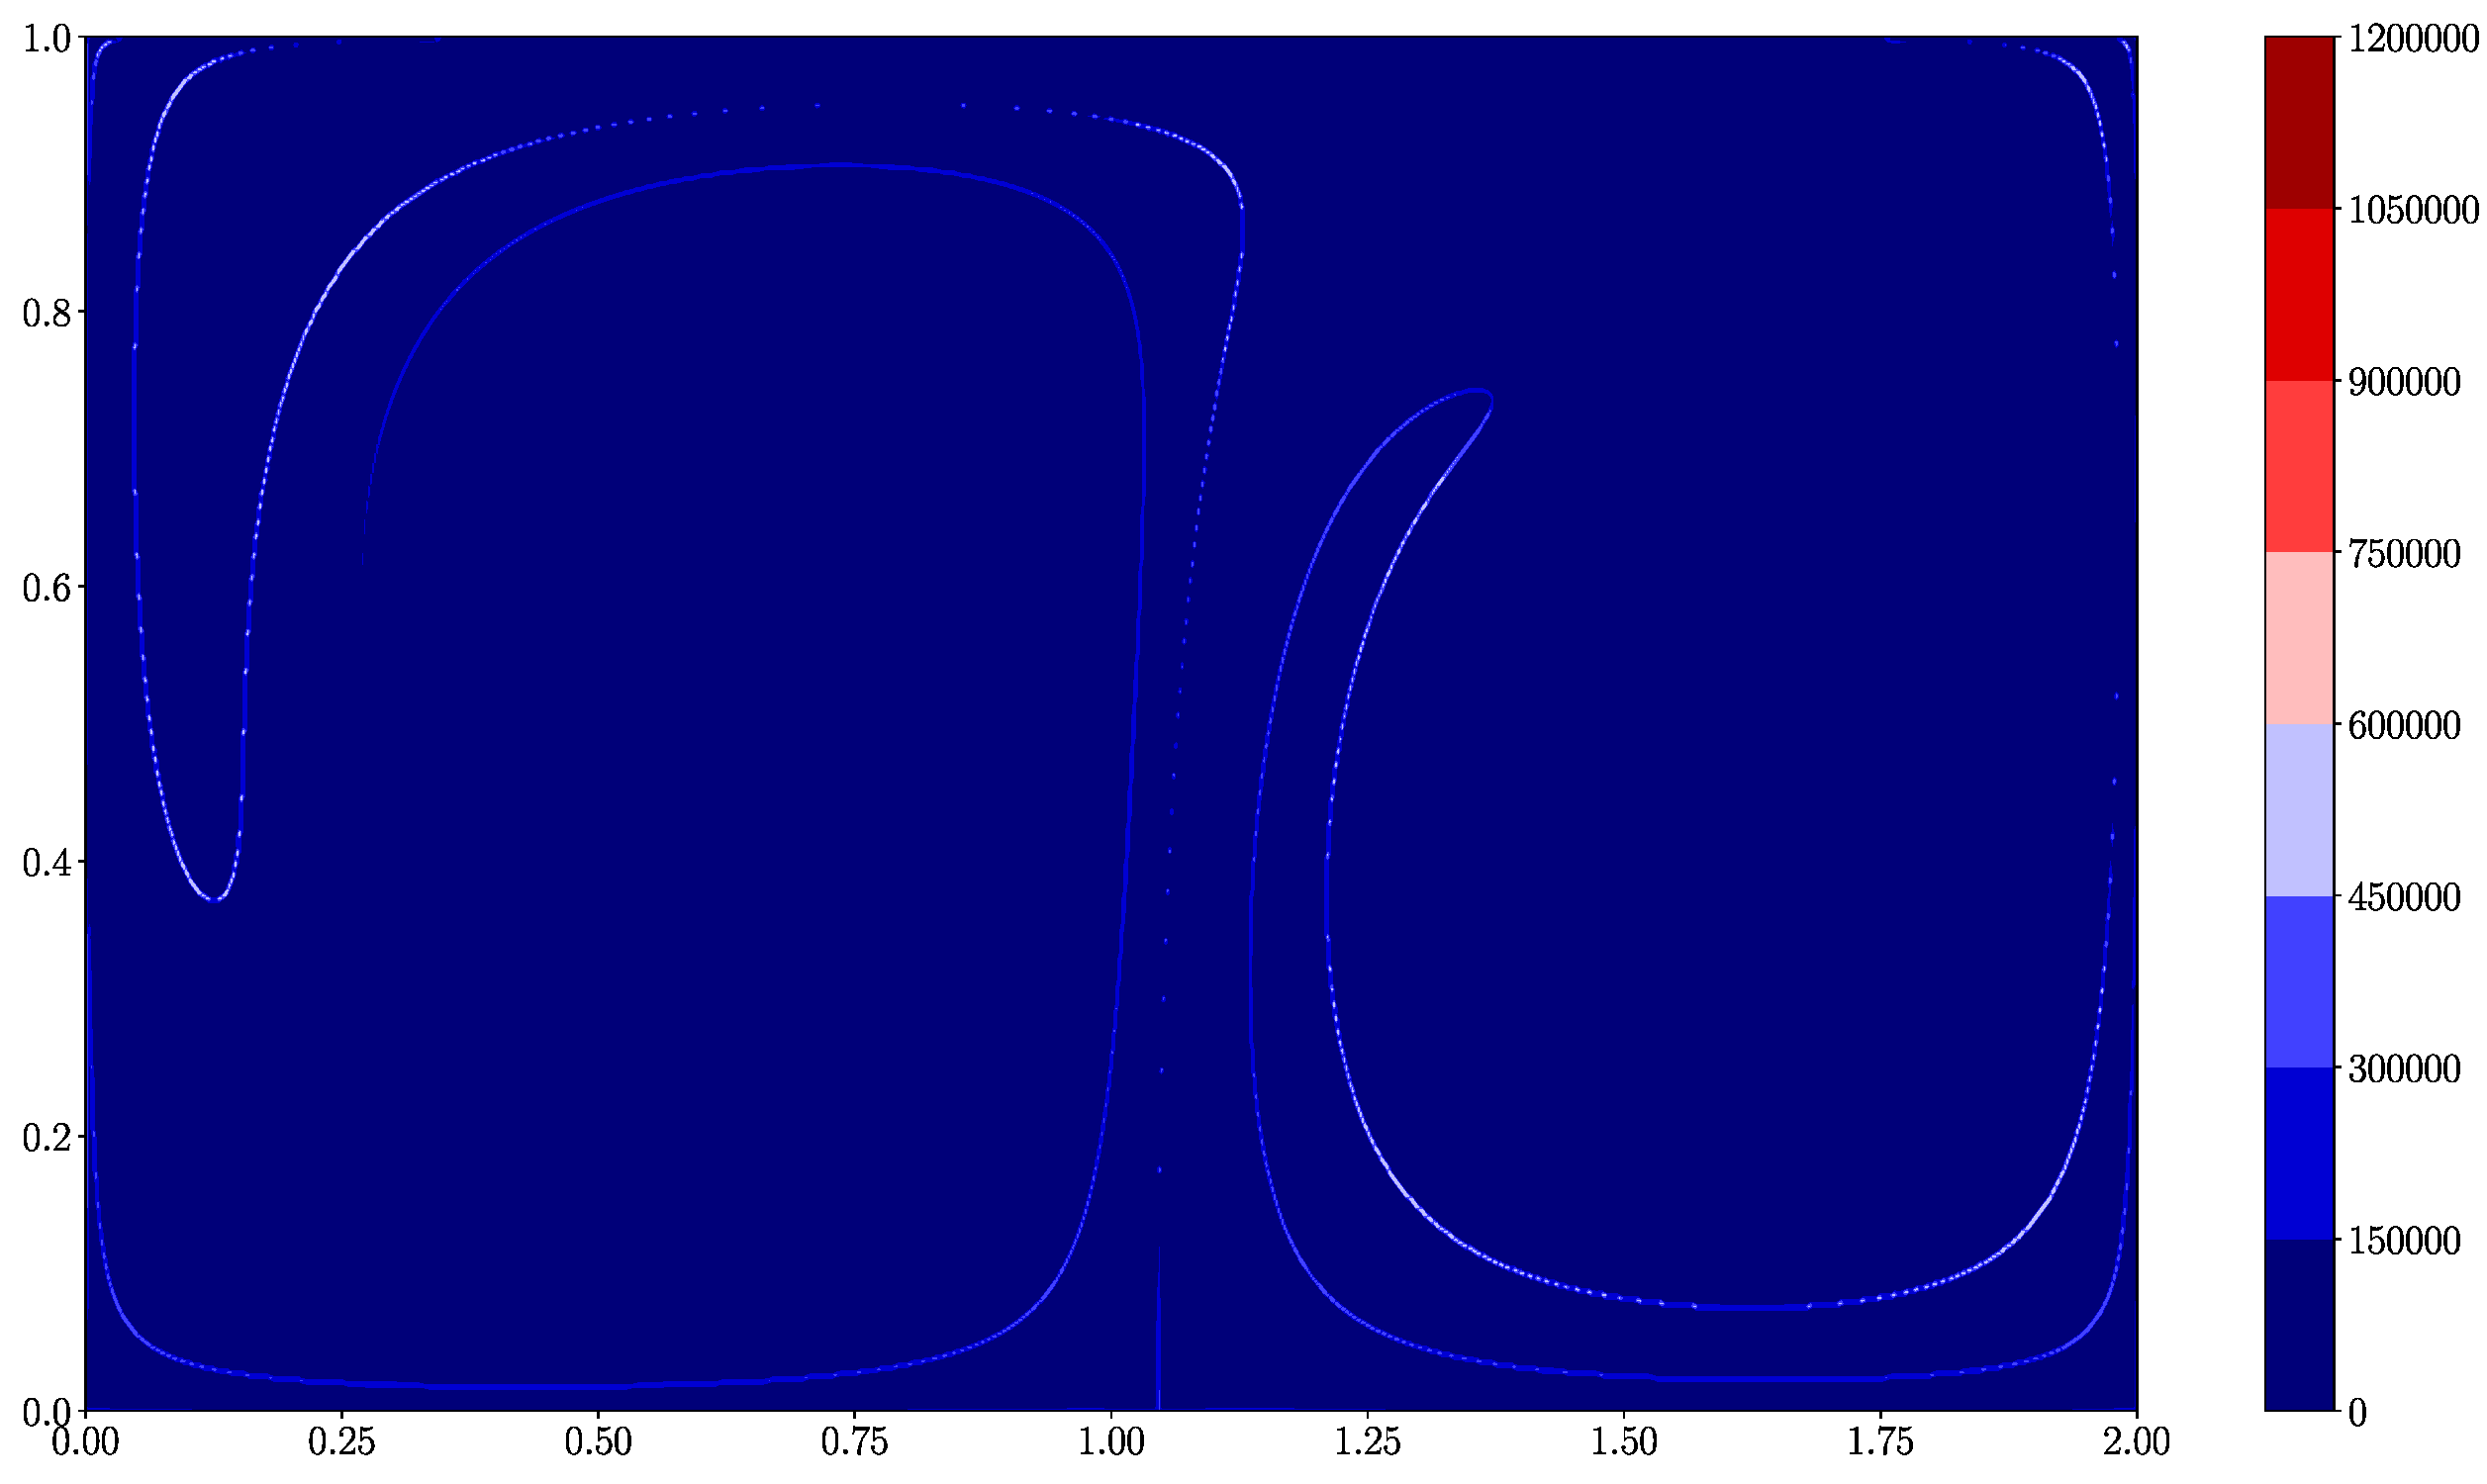
\includegraphics[width=0.75\linewidth,keepaspectratio]{figures/lambda2.pdf}
    \end{subfigure}
    \caption[Contour plots of the FTLE field and $\lambda_{2}(\vct{x}_{0})$
    distribution of the double gyre system]{Contour plots of the FTLE field
    (top) and $\lambda_{2}(\vct{x}_{0})$ (bottom) distribution of the double
    gyre system, given by equation~\eqref{eq:doublegyre}. Due to the different
    scalings, different levels of detail are resolved.
    Most notably, the $\lambda_{2}(\vct{x}_{0})$ contains a thin, patchy ridge
    of extremal values, whereas a similar, albeit continious structure is
    recognizable in the FTLE field. Moreover, the FTLE field exhibits a greater
    amount of detail away from the most prominent ridge than the
    $\lambda_{2}(\vct{x}_{0})$ distribution. Both contours were used, together
    with the domain $\mathcal{U}_{0}$ shown in figure~\ref{fig:u0_domain}, in
    order to select the lines in $\mathcal{L}$, illustrated in figure
    \ref{fig:neighborlcs}.
    }
    \label{fig:ftle_l2}
\end{figure}
